\chapter{Entwicklung des BMS-Algorithmus}\thispagestyle{fancy}


\section{Einf�hrung in das Batterie Management System}
\large{Das Batterie-Management-System ist ein System, welches in der Abteilung Embedded Systems zur �berwachung von Batteriezellen entwickelt wurde. Das BMS misst Spannung, Temperatur und Leitwert an den jeweiligen Zellen. Eine BMS-Platine kann man mit 12 Zellen verbinden und von allen den Spannungswert auslesen. Das BMS wurde in dem Batteriespeicher in Alt Daber im Brandenburg in Betrieb genommen. Es soll vor allem als �berwachungssystem f�r die Firma dienen, damit man die Spannungen und andere Werten kontrollieren kann. Dazu wird, f�r eine bessere �bersichtlichkeit und Orientierung, eine Visualisierung angefertigt. (siehe Abbildung(hier einen Bild Visualisation). Die Daten der jeweiligen Batteriezellen sind in einer unpassenden Anordnung gespeichert. Dies ist der konstruktionsbedingten Verlegung des Kommunikationskabels geschuldet. Dabei ist meine Aufgabe ein Algorithmus zu entwickeln, der die Daten in die richtige, von uns festgestellte, Anordnung sortiert. Damit sollen die Messwerte richtig in der Visualisierung gezeigt werden. }


\section{Erstellung eines BMS-Planes}
\large{Die Batterien sollen mit dem BMS-System belegt werden. Daf�r wurde ein Plan zur Verteilung von BMS Platinen konzipiert. Es existierten mehrere Pl�ne/Versionen, wie die Platinen verbunden werden k�nnen. Wichtige Punkte waren, dass die Kommunikationskabel nicht l�nger als das festgelegte Maximum werden und dass die Batteriezellen mit dem BMS System verbunden werden. Der Plan sollte �bersichtlich sein, weil es der Orientierung in dem EBU dienen soll. Der Plan wurde mit Microsoft Word erstellt. W�hrend einer Gruppenbesprechung wurde die Nummerierung der jeweiligen Teile der EBU festgelegt. In einer EBU gibt es 16 Trog-Verbunde mit jeweils 5 Tr�gen. Ein Trog hat zwei Zellenbl�cke mit jeweils 6 Zellen. Eine Platine kann Werte von zwei Zellenbl�cken messen. Die Platine ist allerdings durch die Kabell�ngen beschr�nkt und reicht nicht �ber einen Trog, das hei�t, dass die Platine die Werte von zwei benachbarten Zellbl�cken messen kann.\\
In dem ersten Plan (siehe Abbildung \ref{Plan_Trogverbund} und \ref{plan_legende}).) ist die Verteilung und Nummerierung zu sehen.\\

\begin{figure}[htbp]
  \centering
     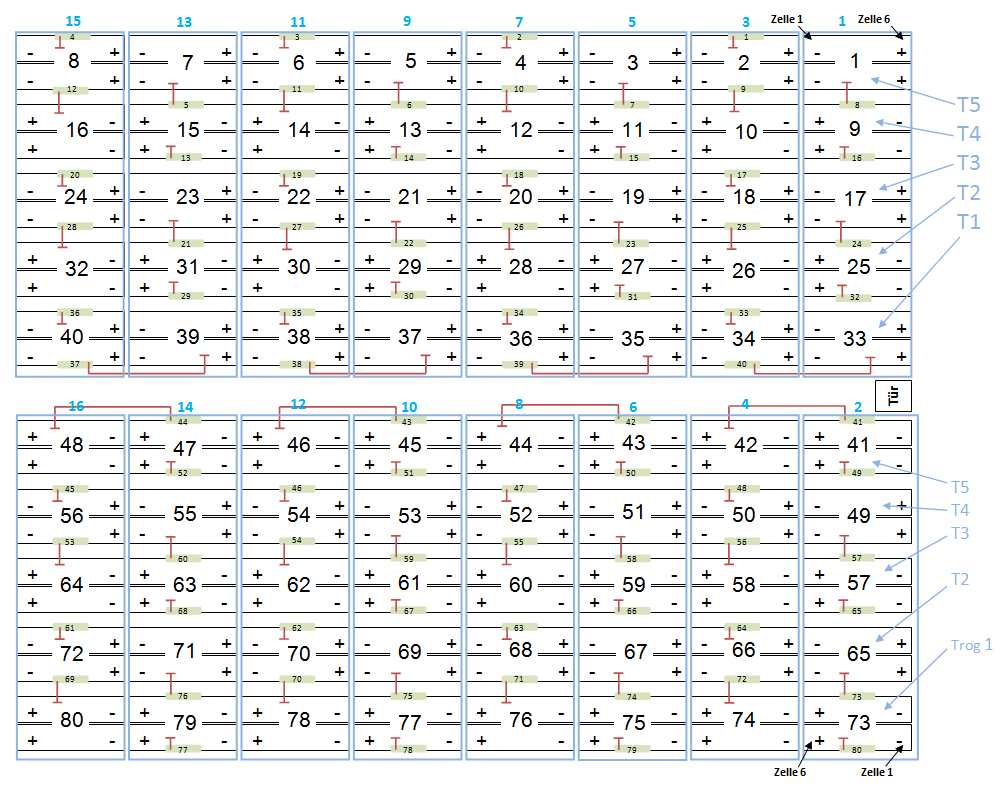
\includegraphics[width=0.99\textwidth]{images/Plan_Trogverbund.png}
  \caption{Plan mit Beschriftung}
  \label{Plan_Trogverbund}
\end{figure}

\begin{figure}[htbp]
  \centering
     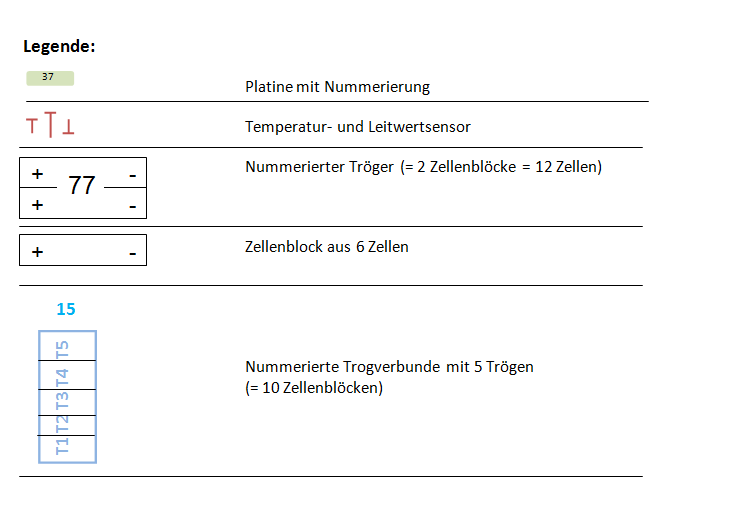
\includegraphics[width=0.8\textwidth]{images/plan_legende.png}
  \caption{Die Legende zum Plan}
  \label{plan_legende}
\end{figure}

In dem zweiten Plan geht es haupts�chlich um die Verkabelung zwischen den BMS-Platinen. Die Platinen wurden mit Kommunikationskabeln verbunden. Dies ist mit blau gekennzeichnet (siehe Abbildung \ref{Montage_plan}).

\begin{figure}[htbp]
  \centering
     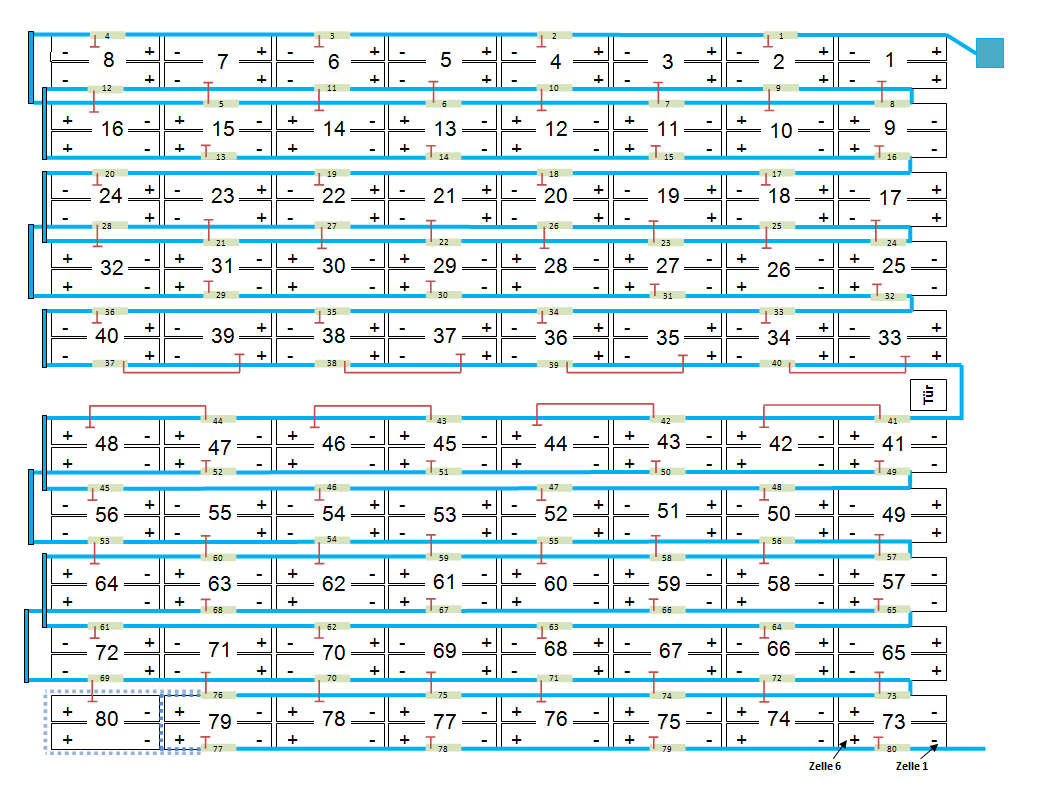
\includegraphics[width=1\textwidth]{images/Montage_plan.png}
  \caption{Verkabelung von Platinen}
  \label{Montage_plan}
\end{figure}
\pagebreak


\section{Entwicklung der Algorithmus}
\large{Zu n�chst wurden Tabellen im Excel erstellt. Die erste Tabelle beinhaltet Informationen zur Verteilung von Platinen. Aus dieser Tabelle sollte man schnell die Nummer der Platine auslesen, welche zum Beispiel die Batteriezelle Nummer 5 des Troges 2 des Trog-Verbundes 11 messen w�rde (siehe Tabellen \ref{tbl:tabelle_excel}). Diese Tabelle dient der besseren Orientierung in einer EBU. \\ 
In der n�chsten Tabelle ist der Zusammenhang zwischen gespeicherte und festgestellte Werte-Indizes beschrieben. Aus dieser Tabelle sollte man zum Beispiel auslesen, dass die Platine Nummer 1 auf die Indizes 0 bis 14 die Werten vom 5. Trog des 1. und 3. Trog-Verbundes speichert. Damit es sortiert wird, muss man die Indizes 0 bis 14 mit die festgesetzte Indizes �berschreiben, in diesem Fall werden es Indizes von 210 bis 215, von 60 bis 65 und drei Indizes 222, 223 und 224 (siehe Tabelle \ref{tbl:example_tabelle_indexing}). Die Visualisierung wird die festgelegte Anordnung anzeigen. \\


\begin{table}
  \caption{Tabelle mit Trogverbund und Reihenordnung}
  \label{tbl:tabelle_excel}
	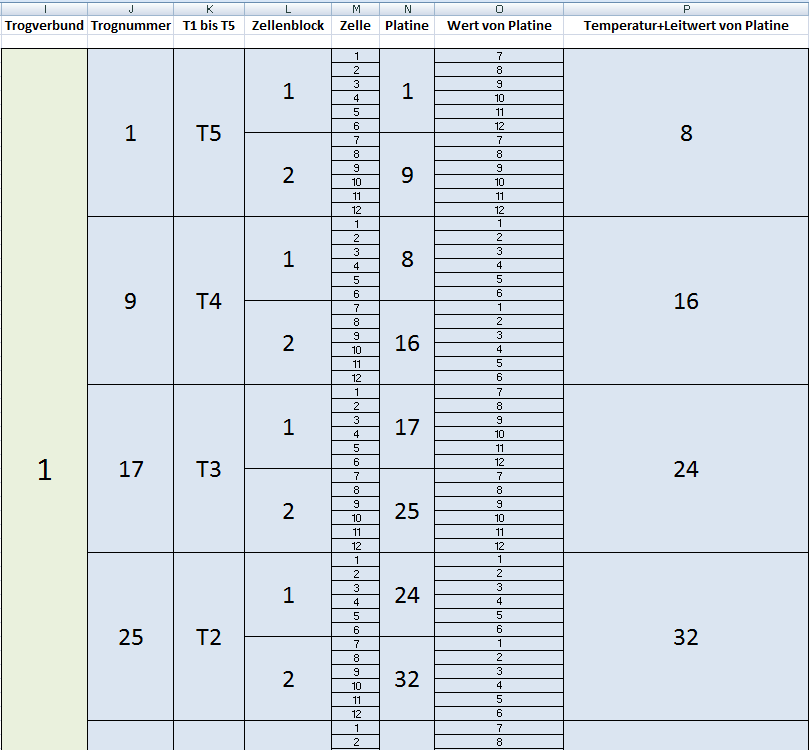
\includegraphics[width=\linewidth]{images/example2_tabelle_excel.png}
\end{table}

% Die Excel Tabellen erstellt, einen System gefunden, sehr viel Berechnen, logische Denken, Spannungswerten, Temperatur, Leitwert, Error

\begin{table}
  \caption{Tabelle mit Indexen}
  \label{tbl:example_tabelle_indexing}
  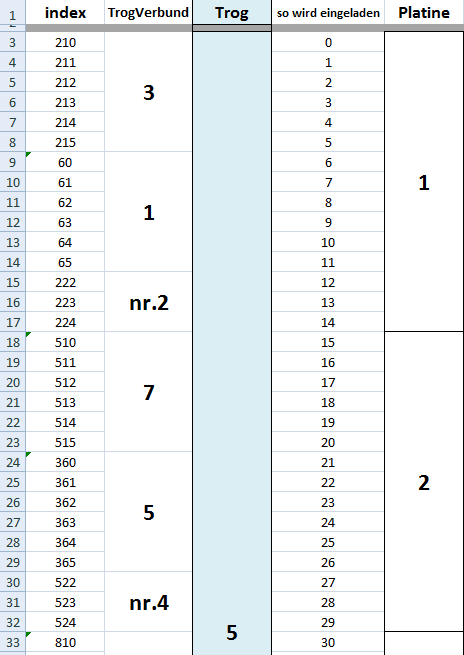
\includegraphics[width=\linewidth]{images/example_tabelle_indexing.png}
\end{table}

Nach dem die Fakten gesammelt wurden, kann man den Algorithmus entwickeln. Man muss die Zusammenh�nge finden und davon allgemeine Regeln bilden. Diese Regeln m�ssen alle Werte-Indizes beschreiben. Dann sind die Regeln zusammengefasst und eine Vereinfachung je nach M�glichkeiten erfolgt. Diese Vereinfachungen wurden mit der Programmiersprache \textit{C} geschrieben. Mit If- und Switch-Operatoren und for-Schleifen wurde die Zuordnung der jeweiligen Werte-Indizes auf die von uns fest gestellten Indizes durchgef�hrt.\\ %siehe Anhang mit dem Algorithmus

Die Visualisierung der BMS Daten erfolgt �ber die B\&R Umgebung, welche die Sprache \textit{ST} benutzt. Der Code in \textit{C} wurde in die Sprache ST umgewandelt und dann in die Umgebung eingesetzt. }%siehe Screenshot von Johann

\pagebreak

\section{Test Durchf�hrung}
\large{Nach der Anwendung der Visualisierung wurde der Algorithmus getestet. Der Test war wurde dabei wie folgt durchgef�hrt: Das was die Visualisierung wiedergibt, muss mit den Werten des Messger�tes verglichen werden. Es wurde an allen Zellen getestet, ob die Werte �bereinstimmen. Der Test zeigte ein positives Ergebnis, das hei�t, dass die Werte auf den richtigen Indizes gespeichert wurden.}

\section{Fazit}
\large{Mit der richtigen Zuordnung der Messwerte kann man den Mitarbeitern oder Kunden zeigen, welche Spannungen an den jeweiligen Batteriezellen anliegen. Auch die Temperaturen und Leitwerte sind damit unter Aufsicht. Die ganze Funktionalit�t wird mittels Visualisierung �berwacht. (Screenshots von Johann)}